
%---------------------- % % % Personnalisation des couleurs % % % ---------- MARRON -------
\definecolor{couleurFonce}{RGB}{110,45,12} % Couleur du Code APOGEE
\definecolor{couleurClaire}{RGB}{200,100,50} % Couleur du fond de la bande
\definecolor{couleurTexte}{RGB}{255,255,255} % Couleur du texte de la bande
%------------------------------------------------------------------------------------------


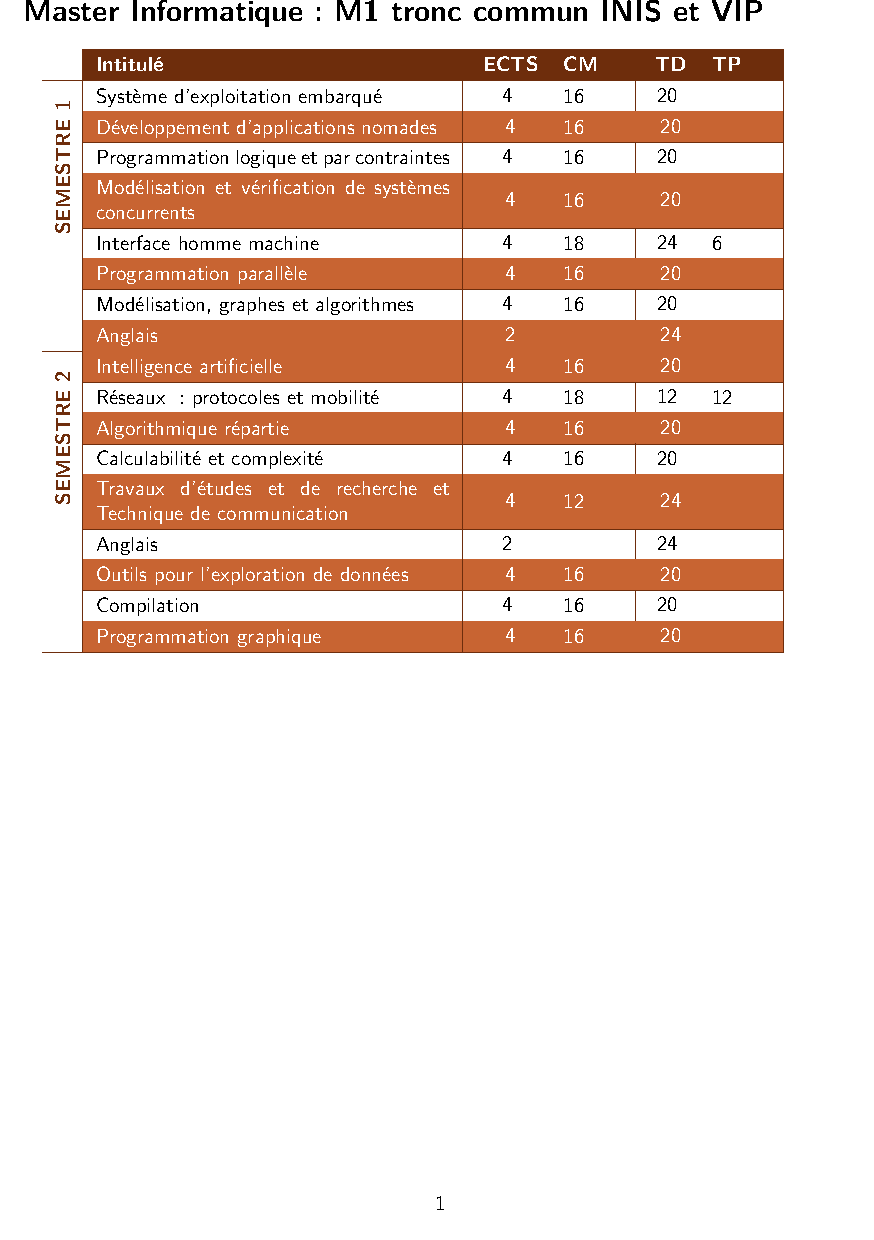
\includepdf[fitpaper,pages=-]{Preambule_Info_MasterINFO_S1S2.pdf}

%==========================================================================================
% Semestre 1
%==========================================================================================
\module[codeApogee={UE 11}, 
titre={Système d\'exploitation embarqué}, 
CODEUE={1}, 
COURS={16}, 
TD={20}, 
TP={}, 
CTD={}, 
TOTAL={36}, 
SEMESTRE={Semestre 1}, 
COEFF={4}, 
ECTS={4}, 
MethodeEval={Contrôle continue et terminal}, 
ModalitesCCSemestreUn={CC et CT}, 
ModalitesCCSemestreDeux={CT}, 
%CalculNFSessionUne={$\frac{(CC+2*CT)}{3}$}, 
%CalculNFSessionDeux={CT}, 
NoteEliminatoire={7}, 
nomPremierResp={Frédéric DABROWSKI}, 
emailPremierResp={Frederic.DABROWSKI@univ-orleans.fr}, 
nomSecondResp={}, 
emailSecondResp={}, 
langue={Français}, 
nbPrerequis={0}, 
descriptionCourte={true}, 
descriptionLongue={true}, 
objectifs={true}, 
ressources={true}, 
bibliographie={false}] 
{
Unité obligatoire 
} 
{
Ce cours porte sur l\'étude des concepts des systèmes d\'exploitation au travers du noyau linux (à la base de nombreux systèmes mobile, en particulier d\'Android).
Un sous-ensemble du noyau linux servira de base à la mise en oeuvre de différents concepts comme la pagination, la segmentation, le multi-tâches, les systèmes de fichiers,...
L\'accent sera mis sur l\'utilisation d\'un noyau linux dans le cadre de la gestion de systèmes nomades.
Des réalisations pratiques impliquant des matériels embarqués seront proposées.
} 
{kkk} 
{\begin{itemize}
\ObjItem Connaissance des principes des systèmes d\'exploitation
\ObjItem Maîtrise des subtilités du noyau linux pour le développement d\'applications
\ObjItem Capacité à modifier un noyau linux pour des applications spécifiques
\ObjItem Capacité à adapter le noyau linux à une plateforme nomade donnée
\end{itemize} 
} 
{Plateforme de cours en ligne pour le M1 Informatique\,: URL}
{Biblio}
 
\vfill

%==========================================================================================
\module[codeApogee={UE 12}, 
titre={Développement d\'applications nomades}, 
CODEUE={1}, 
COURS={16}, 
TD={20}, 
TP={}, 
CTD={}, 
TOTAL={36}, 
SEMESTRE={Semestre 1}, 
COEFF={4}, 
ECTS={4}, 
MethodeEval={Réalisation d\'une application pour mobiles}, 
ModalitesCCSemestreUn={Rapport et soutenance de projet}, 
ModalitesCCSemestreDeux={Rapport et soutenance de projet}, 
%CalculNFSessionUne={$\frac{(CC+2*CT)}{3}$}, 
%CalculNFSessionDeux={CT}, 
NoteEliminatoire={7}, 
nomPremierResp={AbdelAli ED-DBALI}, 
emailPremierResp={AbdelAli.ED-DBALI@univ-orleans.fr}, 
nomSecondResp={}, 
emailSecondResp={}, 
langue={Français}, 
nbPrerequis={1}, 
descriptionCourte={true}, 
descriptionLongue={true}, 
objectifs={true}, 
ressources={true}, 
bibliographie={false}] 
{
Unité obligatoire 
} 
{
\begin{itemize}
\item Architectures et plateformes
\item Développement d\'applications sous Android
\item Développement web pour mobile
\item Sensibilisation au développement sous iOS
\end{itemize}
} 
{Programmation C, C++ ou Java. Notion d\'architecture des ordinateurs.
} 
{\begin{itemize}
\ObjItem Fournir une culture autour de l\'informatique nomade : domaines d\'applications concernés, enjeux, spécificités, possibilités offertes mais également limitations.
\ObjItem Apporter une expérience du développement sur différents systèmes nomades afin de les exploiter le plus efficacement possible.
\end{itemize} 
} 
{Plateforme de cours en ligne pour le M1 Informatique\,: URL} 
{Biblio} 
 
\vfill

%==========================================================================================
\module[codeApogee={UE 13}, 
titre={Programmation logique et par contraintes}, 
CODEUE={1}, 
COURS={16}, 
TD={20}, 
TP={}, 
CTD={}, 
TOTAL={36}, 
SEMESTRE={Semestre 1}, 
COEFF={4}, 
ECTS={4}, 
MethodeEval={Contrôle continue et terminal}, 
ModalitesCCSemestreUn={CC et CT}, 
ModalitesCCSemestreDeux={CT}, 
%CalculNFSessionUne={$\frac{(CC+2*CT)}{3}$}, 
%CalculNFSessionDeux={CT}, 
NoteEliminatoire={7}, 
nomPremierResp={Bich DAO}, 
emailPremierResp={Bich.DAO@univ-orleans.fr}, 
nomSecondResp={}, 
emailSecondResp={}, 
langue={Français}, 
nbPrerequis={1}, 
descriptionCourte={true}, 
descriptionLongue={true}, 
objectifs={true}, 
ressources={true}, 
bibliographie={false}] 
{
Unité obligatoire 
} 
{
\begin{enumerate}
\item La programmation en logique avec Prolog : 
\begin{itemize}
\item point de vue déclaratif
\item résolution SLD, sémantiques opérationnelle et déclarative
\item structure des listes, coupure, négation
\item prédicats d\'ordre supérieur, méta-programmation
\end{itemize}
\item Notion de contraintes et de solveurs de contraintes : études de contraintes de domaines finis, de domaine booléen.
\end{enumerate}
} 
{Logiques mathématiques
} 
{\begin{itemize}
\ObjItem L\'utilisation des langages de Prolog et des solveurs de contraintes intégrés.
\ObjItem Capacité de programmer pour résoudre des problèmes par une approche déclarative en utilisant la logique du premier ordre.
 \end{itemize} 
} 
{Plateforme de cours en ligne pour le M1 Informatique\,: URL} 
{Biblio} 
 
\vfill

%==========================================================================================
\module[codeApogee={UE 14}, 
titre={Modélisation et vérification de systèmes concurrents}, 
CODEUE={1}, 
COURS={16}, 
TD={20}, 
TP={}, 
CTD={}, 
TOTAL={36}, 
SEMESTRE={Semestre 1}, 
COEFF={4}, 
ECTS={4}, 
MethodeEval={Contrôle continue et terminal}, 
ModalitesCCSemestreUn={CC et CT}, 
ModalitesCCSemestreDeux={CT}, 
%CalculNFSessionUne={$\frac{(CC+2*CT)}{3}$}, 
%CalculNFSessionDeux={CT}, 
NoteEliminatoire={7}, 
nomPremierResp={Yohan BOICHUT}, 
emailPremierResp={Yohan.BOICHUT@univ-orleans.fr}, 
nomSecondResp={}, 
emailSecondResp={}, 
langue={Français}, 
nbPrerequis={1}, 
descriptionCourte={true}, 
descriptionLongue={true}, 
objectifs={true}, 
ressources={true}, 
bibliographie={false}] 
{
Unité obligatoire 
} 
{
Ce module introduit le concept de logiques appliquées au contexte de la vérification de systèmes concurrents. Des formules logiques permettent de modéliser les propriétés attendues par un système. Ce système est décrit sous forme de système d\'états/transitions. Le model-checking est une technique permettant de vérifier si une propriété est satisfaite ou non sur un système donné. Dans le cas négatif, une trace du comportement non-souhaité du système est retournée par cette technique. Pour mieux comprendre cette application des logiques, ce module débute par une étude des logiques monadiques du 2nd ordre sur les mots finis et infinis. Ce cadre constitue les fondements de la technique de Model-Checking. La transformation d\'une formule en automate de mots finis ou automate de mots infinis est étudiée en profondeur. Ainsi, savoir si une formule f est satisfaite sur un langage L revient à calculer l\'automate de la négation de f puis calculer l\'intersection avec le langage L. Une intersection vide signifie que la négation de f n\'est pas satisfaite, et donc que f est satisfaite. D\'une intersection non vide, nous en déduisons que la formule n\'est pas satisfaite et de l\'intersection, nous pouvons extraire un mot témoin. Une fois les fondements théoriques établis, les logiques temporelles usuelles LTL et CTL sont étudiées. Dans le cadre de LTL, l\'outil de vérification SPIN mènera les étudiants à modéliser les systèmes sous forme de procéssus et les propriétés attendues de ce système sous forme de formules logiques.
} 
{Notions élémentaires en logique, théorie des langages 
} 
{
\begin{itemize}\ObjItem Maîtriser et comprendre une technique de vérification,
 \ObjItem modéliser en logique les propriétés attendues d\'un système 
 \end{itemize} 
} 
{Plateforme de cours en ligne pour le M1 Informatique\,: URL} 
{Biblio} 
 
\vfill

%==========================================================================================
\module[codeApogee={UE 15}, 
titre={Interface homme machine}, 
CODEUE={1}, 
COURS={18}, 
TD={24}, 
TP={6}, 
CTD={}, 
TOTAL={48}, 
SEMESTRE={Semestre 1}, 
COEFF={4}, 
ECTS={4}, 
MethodeEval={Contrôle continue et terminal}, 
ModalitesCCSemestreUn={CC et CT}, 
ModalitesCCSemestreDeux={CT}, 
%CalculNFSessionUne={$\frac{(CC+2*CT)}{3}$}, 
%CalculNFSessionDeux={CT}, 
NoteEliminatoire={7}, 
nomPremierResp={Frédéric MOAL}, 
emailPremierResp={Frederic.MOAL@univ-orleans.fr}, 
nomSecondResp={}, 
emailSecondResp={}, 
langue={Français}, 
nbPrerequis={1}, 
descriptionCourte={true}, 
descriptionLongue={true}, 
objectifs={true}, 
ressources={true}, 
bibliographie={false}] 
{
Unité obligatoire 
} 
{
\begin{itemize}
\item Principes de la programmation événementielle, le modèle MVC
\item Définition et programmation des interfaces graphiques en client {\it lourd}
\item Illustration et mise en oeuvre avec le langage Java/SWING
\item Architectures des interfaces Web (JSP/servlets), le modèle MVC 2
\item Utilisation des frameworks Javascript / Exemple de GWT (Google Web Toolkit)
\item Les interfaces des terminaux portables / Exemple d\'Android
\end{itemize}
} 
{Programmation Java, maîtrise de la programmation orientée objet 
} 
{\begin{itemize}
\ObjItem Comprendre les architectures Modèle Vue Contrôleur.
\ObjItem Maîtriser le développement et la maintenance d\'IHM pour les architectures clients légers et clients lourds.
\end{itemize} 
} 
{Plateforme de cours en ligne pour le M1 Informatique\,: URL} 
{Biblio} 
 
\vfill

%==========================================================================================
\module[codeApogee={UE 16}, 
titre={Programmation parallèle}, 
CODEUE={1}, 
COURS={16}, 
TD={20}, 
TP={}, 
CTD={}, 
TOTAL={36}, 
SEMESTRE={Semestre 1}, 
COEFF={4}, 
ECTS={4}, 
MethodeEval={Contrôle continue et terminal}, 
ModalitesCCSemestreUn={CC et CT}, 
ModalitesCCSemestreDeux={CT}, 
%CalculNFSessionUne={$\frac{(CC+2*CT)}{3}$}, 
%CalculNFSessionDeux={CT}, 
NoteEliminatoire={7}, 
nomPremierResp={Sophie ROBERT}, 
emailPremierResp={Sophie.ROBERT@univ-orleans.fr}, 
nomSecondResp={}, 
emailSecondResp={}, 
langue={Français}, 
nbPrerequis={1}, 
descriptionCourte={true}, 
descriptionLongue={true}, 
objectifs={true}, 
ressources={true}, 
bibliographie={false}] 
{
Unité obligatoire 
} 
{
Extrêmement importants dans la plupart des domaines scientifiques, le calcul scientifique et la simulation numérique ont également pris une grande place dans des applications technologiques. Ils sont utilisés pour concevoir, optimiser et réduire les risques de développement dans tous les domaines de l\'activité économique (simulations de phénomènes physiques, biologiques, économiques... , maquettes numériques). Ce module aborde les bases de la programmation parallèle de machines à mémoire répartie :
\begin{itemize}
\item Architectures parallèles
\item Algorithmique parallèle
\item Programmation parallèle impérative par passage de messages
\item Programmation répartie modulaire et politiques de synchronisation fines
\end{itemize}
} 
{Programmation impérative, utilisation d\'un système unix, outils de développements
} 
{Compétences pour la programmation d\'applications pour supercalculateurs à mémoire répartie.
Ce module est un pré-requis pour les modules de M2 "Programmation multi-coeurs" et "Visualisation avancée". 
} 
{Plateforme de cours en ligne pour le M1 Informatique\,: URL} 
{Biblio} 
 
\vfill

%==========================================================================================
\module[codeApogee={UE 17}, 
titre={Modélisation, graphes et algorithmes}, 
CODEUE={1}, 
COURS={16}, 
TD={20}, 
TP={}, 
CTD={}, 
TOTAL={36}, 
SEMESTRE={Semestre 1}, 
COEFF={4}, 
ECTS={4}, 
MethodeEval={Contrôle continue et terminal}, 
ModalitesCCSemestreUn={CC et CT}, 
ModalitesCCSemestreDeux={CT}, 
%CalculNFSessionUne={$\frac{(CC+2*CT)}{3}$}, 
%CalculNFSessionDeux={CT}, 
NoteEliminatoire={7}, 
nomPremierResp={Ioan TODINCA}, 
emailPremierResp={Ioan.TODINCA@univ-orleans.fr}, 
nomSecondResp={Mathieu LIEDLOFF}, 
emailSecondResp={Mathieu.LIEDLOFF@univ-orleans.fr}, 
langue={Français}, 
nbPrerequis={1}, 
descriptionCourte={true}, 
descriptionLongue={true}, 
objectifs={true}, 
ressources={true}, 
bibliographie={false}] 
{
Unité obligatoire 
} 
{
L\'enseignement aborde à la fois des aspects algorithmiques d\'optimisation combinatoire avec des techniques de résolution polynomiale (flots et réseaux de transport, problèmes de postier chinois...), d\'approximation (voyageur de commerce...) et heuristiques pour des problèmes difficiles comme la coloration ou le stable maximum) et des aspects de modélisation des réseaux d\'interconnexion et de problèmes d\'algorithmique distribuée.
} 
{Algorithmique élémentaire sur les graphes, programmation linéaire
} 
{\begin{itemize}
\ObjItem Savoir modéliser et résoudre des problèmes d\'optimisation sur les graphes.
\end{itemize} 
} 
{Plateforme de cours en ligne pour le M1 Informatique\,: URL} 
{Biblio} 
 
\vfill

%==========================================================================================
\module[codeApogee={UE 18}, 
titre={Anglais}, 
CODEUE={1}, 
COURS={}, 
TD={24}, 
TP={}, 
CTD={}, 
TOTAL={24}, 
SEMESTRE={Semestre 1}, 
COEFF={2}, 
ECTS={2}, 
MethodeEval={Contrôle continue et terminal}, 
ModalitesCCSemestreUn={CC et CT}, 
ModalitesCCSemestreDeux={CT}, 
%CalculNFSessionUne={$\frac{(CC+2*CT)}{3}$}, 
%CalculNFSessionDeux={CT}, 
NoteEliminatoire={7}, 
nomPremierResp={Cédric SARRE}, 
emailPremierResp={Cedric.SARRE@univ-orleans.fr}, 
nomSecondResp={}, 
emailSecondResp={}, 
langue={Français}, 
nbPrerequis={1}, 
descriptionCourte={true}, 
descriptionLongue={true}, 
objectifs={true}, 
ressources={true}, 
bibliographie={false}] 
{
Unité obligatoire 
} 
{
Etudes des techniques de présentation orale : amélioration de la prononciation, organisation du discours, guidage de l\'auditoire, élaboration d\'aides visuelles, etc.
} 
{Anglais non professionnel
} 
{\begin{itemize}
\ObjItem S\'exprimer couramment et efficacement dans le domaine de la spécialité.
\end{itemize} 
} 
{Page du département des langues\,: {\tt http://www.univ-orleans.fr/sciences/?page=12}} 
{Biblio} 
 
\vfill

%==========================================================================================
% Semestre 2
%==========================================================================================

\module[codeApogee={UE 21}, 
titre={Intelligence artificielle}, 
CODEUE={1}, 
COURS={16}, 
TD={20}, 
TP={}, 
CTD={}, 
TOTAL={36}, 
SEMESTRE={Semestre 2}, 
COEFF={4}, 
ECTS={4}, 
MethodeEval={Contrôle continue et terminal}, 
ModalitesCCSemestreUn={CC et CT}, 
ModalitesCCSemestreDeux={CT}, 
%CalculNFSessionUne={$\frac{(CC+2*CT)}{3}$}, 
%CalculNFSessionDeux={CT}, 
NoteEliminatoire={7}, 
nomPremierResp={Matthieu EXBRAYAT}, 
emailPremierResp={Matthieu.EXBRAYAT@univ-orleans.fr}, 
nomSecondResp={}, 
emailSecondResp={}, 
langue={Français}, 
nbPrerequis={1}, 
descriptionCourte={true}, 
descriptionLongue={true}, 
objectifs={true}, 
ressources={true}, 
bibliographie={false}] 
{
Unité obligatoire 
} 
{
\begin{itemize}
\item Introduction à l\'Intelligence Artificielle
\item Résolution de problèmes : modélisation d\'un problème, algorithmes de recherche non informés (largeur, profondeur, ...) et informés (meilleur d\'abord, A*, ...) 
\item Modélisation des connaissances et inférence : représentations logiques et représentations de connaissances incertaines.
\end{itemize}
Dans ce module, sont abordées des techniques fondamentales pour la résolution de problèmes complexes, fondées soit sur la modélisation  du problème par un graphe d\'états,
soit sur la représentation des connaissances sous-jacentes. On peut citer comme domaines d\'application les problèmes d\'aide à la décision,
mais aussi par exemple la  constitution de mémoires d\'entreprises.
} 
{Programmation en logique 
} 
{
\begin{itemize}
\ObjItem Savoir modéliser un problème qui fait appel à des techniques de l\'intelligence artificielle.
\end{itemize}
} 
{Plateforme de cours en ligne pour le M1 Informatique\,: URL} 
{Biblio} 
 
\vfill

%==========================================================================================
\module[codeApogee={UE 22}, 
titre={Réseaux : protocoles et mobilité}, 
CODEUE={1}, 
COURS={18}, 
TD={12}, 
TP={12}, 
CTD={}, 
TOTAL={42}, 
SEMESTRE={Semestre 2}, 
COEFF={4}, 
ECTS={4}, 
MethodeEval={Contrôle continue et terminal}, 
ModalitesCCSemestreUn={CC et CT}, 
ModalitesCCSemestreDeux={CT}, 
%CalculNFSessionUne={$\frac{(CC+2*CT)}{3}$}, 
%CalculNFSessionDeux={CT}, 
NoteEliminatoire={7}, 
nomPremierResp={AbdelAli ED-DBALI}, 
emailPremierResp={AbdelAli.ED-DBALI@univ-orleans.fr}, 
nomSecondResp={}, 
emailSecondResp={}, 
langue={Français}, 
nbPrerequis={1}, 
descriptionCourte={true}, 
descriptionLongue={true}, 
objectifs={true}, 
ressources={true}, 
bibliographie={false}] 
{
Unité obligatoire 
} 
{
\begin{itemize}
\item Spécification de protocoles (à l\'aide des automates d\'états finis étendus)
\item Etude détaillée des protocoles : TCP, DHCP et NAT
\item Les réseaux mobiles : Etude du protocole 802.11 (wifi), éléments de sécurité dans les réseaux sans fils (WEP, WPA, ...),
autres protocoles sans fils (Bluetooth, WiMax, GPRS, ...), mobilité
\end{itemize}
} 
{Protocole IP, routage (programme du module "réseaux 1" de licence 3)
} 
{ 
\begin{itemize}
\ObjItem Comprendre et réaliser des spécifications de protocoles réseaux.
\ObjItem Installer, configurer et sécuriser un réseau local hétérogène (avec du filaire et du WiFi) ouvert sur Internet.
\end{itemize} 
} 
{Plateforme de cours en ligne pour le M1 Informatique\,: URL} 
{Biblio} 
 
\vfill

%==========================================================================================
\module[codeApogee={UE 23}, 
titre={Algorithmique répartie}, 
CODEUE={1}, 
COURS={16}, 
TD={20}, 
TP={}, 
CTD={}, 
TOTAL={36}, 
SEMESTRE={Semestre 2}, 
COEFF={4}, 
ECTS={4}, 
MethodeEval={Contrôle continue et terminal}, 
ModalitesCCSemestreUn={CC et CT}, 
ModalitesCCSemestreDeux={CT}, 
%CalculNFSessionUne={$\frac{(CC+2*CT)}{3}$}, 
%CalculNFSessionDeux={CT}, 
NoteEliminatoire={7}, 
nomPremierResp={Frédéric DABROWSKI}, 
emailPremierResp={Frederic.DABROWSKI@univ-orleans.fr}, 
nomSecondResp={}, 
emailSecondResp={}, 
langue={Français}, 
nbPrerequis={1}, 
descriptionCourte={true}, 
descriptionLongue={true}, 
objectifs={true}, 
ressources={true}, 
bibliographie={false}] 
{
Unité obligatoire 
} 
{
Ce module vise à sensibiliser les étudiants aux problèmes particuliers qui se posent lorsque les processus participant à une application s\'exécutent sur des sites distants.
Le modèle de répartition auquel nous nous intéressons ici est celui de la communication par message.
Les solutions existantes à différents problèmes classiques dans ce contexte seront présentéesÊ:
gestion du temps, réalisation de l\'exclusion mutuelle, détection de la terminaison de l\'application, etc.
Il aborde les thèmes suivants communication entre site (algorithme de parcours), causalité en l\'absence d\'horloge globale, mécanismes d\'horloges logiques,
calcul d\'état global, élection, terminaison.
} 
{Programmation parallèle
} 
{Sensibiliser les étudiants aux problèmes posés par la programmation d\'applications réparties. 
} 
{Plateforme de cours en ligne pour le M1 Informatique\,: URL} 
{Biblio} 
 
\vfill

%==========================================================================================
\module[codeApogee={UE 24}, 
titre={Calculabilité et complexité}, 
CODEUE={1}, 
COURS={16}, 
TD={20}, 
TP={}, 
CTD={}, 
TOTAL={36}, 
SEMESTRE={Semestre 2}, 
COEFF={4}, 
ECTS={4}, 
MethodeEval={Contrôle continue et terminal}, 
ModalitesCCSemestreUn={CC et CT}, 
ModalitesCCSemestreDeux={CT}, 
%CalculNFSessionUne={$\frac{(CC+2*CT)}{3}$}, 
%CalculNFSessionDeux={CT}, 
NoteEliminatoire={7}, 
nomPremierResp={Mathieu LIEDLOFF}, 
emailPremierResp={Mathieu.LIEDLOFF@univ-orleans.fr}, 
nomSecondResp={}, 
emailSecondResp={}, 
langue={Français}, 
nbPrerequis={1}, 
descriptionCourte={true}, 
descriptionLongue={true}, 
objectifs={true}, 
ressources={true}, 
bibliographie={false}] 
{
Unité obligatoire.
} 
{
\begin{itemize}
\item Définition d\'un problème, représentation des données et des résultats. Approche mécanique du calcul, Machine de Turing. Approche inductive, fonction primitive et mu récursives. Equivalence entre les deux modèles et plus généralement Thèse de Church-Turing. Problème indécidables et semi-décidables. Problème de la halte. Réduction entre problèmes.
\item Calcul d\'une machine sur une entrée, notion de ressource et de coût (temps ou espace) d\'une exécution. Complexité d\'un algorithme. Difficulté de comparer les algorithmes, approche asymptotique. Notion de complexité d\'un programme. Class de complexité P. Définition de NP par certificat et non déterministe. Réduction polynomiale entre problèmes. Question P=NP.
\end{itemize} 
} 
{\begin{itemize}
\item Complexité des algorithmes.
\item Théorie des langages.
\end{itemize} 
} 
{\begin{itemize}
\ObjItem Comprendre la relative indifférence des problèmes par rapport à une machine comme un langage de programmation.
\ObjItem Connaître les limites -en terme de problème et non d\'algorithme- de ce que l\'on peut calculer dans l\'absolu (calculabilité) comme dans la pratique (complexité).
\end{itemize} 
} 
{Plateforme de cours en ligne pour le M1 Informatique\,: URL} 
{Biblio} 
 
\vfill

%==========================================================================================
\module[codeApogee={UE 25}, 
titre={Travaux d\'études et de recherche et Technique de communication}, 
CODEUE={1}, 
COURS={12}, 
TD={24}, 
TP={}, 
CTD={}, 
TOTAL={36}, 
SEMESTRE={Semestre 2}, 
COEFF={4}, 
ECTS={4}, 
MethodeEval={Contrôle continue et terminal}, 
ModalitesCCSemestreUn={CC et CT}, 
ModalitesCCSemestreDeux={CT}, 
%CalculNFSessionUne={$\frac{(CC+2*CT)}{3}$}, 
%CalculNFSessionDeux={CT}, 
NoteEliminatoire={7}, 
nomPremierResp={Jean-Michel COUVREUR}, 
emailPremierResp={Jean-Michel.COUVREUR@univ-orleans.fr}, 
nomSecondResp={AbdelAli ED-DBALI}, 
emailSecondResp={AbdelAli.ED-DBALI@univ-orleans.fr}, 
langue={Français}, 
nbPrerequis={1}, 
descriptionCourte={true}, 
descriptionLongue={true}, 
objectifs={true}, 
ressources={true}, 
bibliographie={false}] 
{
Unité obligatoire composée de deux domaines séparés.
} 
{
L\'unité "Travaux d\'études et de recherche" (TER) est articulée autour de trois axes :
\begin{itemize}
\item génie logiciel: analyse des besoins et élaboration du cahier des charges, conception et implémentation, test, réalisation d\'une documentation et d\'une distribution portable, travail en équipe. 
\item pratique scientifique : recherche et analyse de l\'existant, justifications, critiques du travail réalisé, assimilation de nouveaux concepts dans la discipline ou transdisciplinaires.
\item recherche documentaire : Manipulation des bases de données et des catalogues disponibles au service commun de la documentation.
\end{itemize}
L\'unité "Technique de communication" vise l\'apprentissage des principales techniques de communication liées à la gestion de projetÊ: technique de réunion, gestion des relations entre personnes, conduite de projet.
} 
{Pour la partie TER : différents aspects de la programmation (impérative, fonctionnelle et par objets).
} 
{\begin{itemize}
\ObjItem TER
\begin{itemize}
\item Mise en pratique de principes et de techniques étudiés dans les unités d\'enseignement,
\item acquisition d\'une expérience de génie logiciel, application d\'une pratique scientifique
\end{itemize}
\ObjItem Technique de communication
\begin{itemize}
\item Comprendre l\'importance des relations humaines dans un projet.
\item Apprendre à maîtriser les problèmes humains dans un projet.
\end{itemize}
\end{itemize} 
} 
{Plateforme de cours en ligne pour le M1 Informatique\,: URL} 
{Biblio} 
 
\vfill

%==========================================================================================
\module[codeApogee={UE 26}, 
titre={Anglais}, 
CODEUE={1}, 
COURS={}, 
TD={24}, 
TP={}, 
CTD={}, 
TOTAL={24}, 
SEMESTRE={Semestre 2}, 
COEFF={2}, 
ECTS={2}, 
MethodeEval={Contrôle continue et terminal}, 
ModalitesCCSemestreUn={CC et CT}, 
ModalitesCCSemestreDeux={CT}, 
%CalculNFSessionUne={$\frac{(CC+2*CT)}{3}$}, 
%CalculNFSessionDeux={CT}, 
NoteEliminatoire={7}, 
nomPremierResp={Cédric SARRE}, 
emailPremierResp={Cedric.SARRE@univ-orleans.fr}, 
nomSecondResp={}, 
emailSecondResp={}, 
langue={Français}, 
nbPrerequis={1}, 
descriptionCourte={true}, 
descriptionLongue={true}, 
objectifs={true}, 
ressources={true}, 
bibliographie={false}] 
{
Unité obligatoire qui fait suite à l\'unité UE18 : Anglais du premier semestre.
}
{
Etudes des techniques de présentation orale : amélioration de la prononciation, organisation du discours, guidage de l\'auditoire, élaboration d\'aides visuelles, etc.
} 
{Anglais non professionnel
} 
{\begin{itemize}
\ObjItem S\'exprimer couramment et efficacement dans le domaine de la spécialité.
\end{itemize} 
} 
{Page du département des langues\,: http://www.univ-orleans.fr/sciences/?page=12} 
{Biblio} 

 
\vfill

%==========================================================================================
\module[codeApogee={UE 27 }, 
titre={Outils pour l\'exploration de données}, 
CODEUE={1}, 
COURS={16}, 
TD={20}, 
TP={}, 
CTD={}, 
TOTAL={36}, 
SEMESTRE={Semestre 2}, 
COEFF={4}, 
ECTS={4}, 
MethodeEval={Contrôle continue et terminal}, 
ModalitesCCSemestreUn={CC et CT}, 
ModalitesCCSemestreDeux={CT}, 
%CalculNFSessionUne={$\frac{(CC+2*CT)}{3}$}, 
%CalculNFSessionDeux={CT}, 
NoteEliminatoire={7}, 
nomPremierResp={Christel VRAIN}, 
emailPremierResp={Christel.VRAIN@univ-orleans.fr}, 
nomSecondResp={}, 
emailSecondResp={}, 
langue={Français}, 
nbPrerequis={0}, 
descriptionCourte={true}, 
descriptionLongue={true}, 
objectifs={true}, 
ressources={true}, 
bibliographie={false}] 
{
Fait partie des 2 UE à choisir parmi les 3 UE (UE 27, UE 28 et UE 29)} 
{
\begin{itemize}
\item Apprentissage et développement en langage R
\item Notions élémentaires de probabilités : variables aléatoires, loi, espérance, variance, probabilité conditionnelle
\item Statistiques descriptives :
 \begin{itemize}
 \item Indicateurs de tendance centrale, de dispersion et de forme (médiane, quantiles, moyenne, mode, variance et écart-type), tableau de contingence,
 \item Contrôle de la qualité des données (valeurs aberrantes, données manquantes, ..)
 \item Coefficient de corrélation, matrice de corrélation
 \end{itemize} 
\item Analyse de données: analyse en composantes principales, analyse des correspondances, analyse discriminante
\end{itemize} 
} 
{} 
{\begin{itemize}
\ObjItem Etre capable d\'effectuer tous les traitements simples sur un jeu de données.
\ObjItem Etre capable de produire une étude descriptive et d\'en interpréter les résultats.
\ObjItem Connaître les principes de l\'analyse et visualisation du nuage d\'individus/de variables, interpréter les résultats.
\end{itemize} 
} 
{Plateforme de cours en ligne pour le M1 Informatique\,: URL} 
{Biblio} 
 
\vfill

%==========================================================================================
\module[codeApogee={UE 28 }, 
titre={Compilation}, 
CODEUE={1}, 
COURS={16}, 
TD={20}, 
TP={}, 
CTD={}, 
TOTAL={36}, 
SEMESTRE={Semestre 2}, 
COEFF={4}, 
ECTS={4}, 
MethodeEval={Contrôle continue et terminal}, 
ModalitesCCSemestreUn={CC et CT}, 
ModalitesCCSemestreDeux={CT}, 
%CalculNFSessionUne={$\frac{(CC+2*CT)}{3}$}, 
%CalculNFSessionDeux={CT}, 
NoteEliminatoire={7}, 
nomPremierResp={Jean-Michel COUVREUR}, 
emailPremierResp={Jean-Michel.COUVREUR@univ-orleans.fr}, 
nomSecondResp={}, 
emailSecondResp={}, 
langue={Français}, 
nbPrerequis={1}, 
descriptionCourte={true}, 
descriptionLongue={true}, 
objectifs={true}, 
ressources={true}, 
bibliographie={false}] 
{
Fait partie des 2 UE à choisir parmi les 3 UE (UE 27, UE 28 et UE 29) 
} 
{
\begin{itemize}
\item Conception d\'un compilateur : de la théorie à la pratique.
\item Analyse syntaxique et sémantique.
\item Traitement des erreurs.
\item Génération de code.
\item Traitement des types complexes.
\item Fonctions et procédures.
\item Edition de liens.
\end{itemize}
} 
{Programmation impérative, Programmation fonctionnelle, Programmation par objets. Théorie des langages.} 
{\begin{itemize}
\ObjItem Savoir utiliser les générateurs d\'analyseurs.
\ObjItem Maitriser les mécanismes de transduction d\'un langage de haut niveau vers un assembleur.
\end{itemize} 
} 
{Plateforme de cours en ligne pour le M1 Informatique\,: URL} 
{Biblio} 
 
\vfill

%==========================================================================================
\module[codeApogee={UE 29}, 
titre={Programmation graphique}, 
CODEUE={1}, 
COURS={16}, 
TD={20}, 
TP={}, 
CTD={}, 
TOTAL={36}, 
SEMESTRE={Semestre 2}, 
COEFF={4}, 
ECTS={4}, 
MethodeEval={Contrôle continue et terminal}, 
ModalitesCCSemestreUn={CC et CT}, 
ModalitesCCSemestreDeux={CT}, 
%CalculNFSessionUne={$\frac{(CC+2*CT)}{3}$}, 
%CalculNFSessionDeux={CT}, 
NoteEliminatoire={7}, 
nomPremierResp={Sophie ROBERT}, 
emailPremierResp={Sophie.ROBERT@univ-orleans.fr}, 
nomSecondResp={Rachid JENNANE}, 
emailSecondResp={Rachid.JENNANE@univ-orleans.fr}, 
langue={Français}, 
nbPrerequis={1}, 
descriptionCourte={true}, 
descriptionLongue={true}, 
objectifs={true}, 
ressources={true}, 
bibliographie={false}] 
{
Fait partie des 2 UE à choisir parmi les 3 UE (UE 27, UE 28 et UE 29) 
} 
{
\begin{itemize}
\item Pipeline graphique et introduction à OpenGL. La synthèse d\'images et la visualisation sont des domaines importants en informatique qui s\'appuient sur leur propre paradigme de développement. Dans cette première partie, ce module présentera le pipeline graphique afin de connaître le fonctionnement d\'une carte graphique simple. Ensuite, la programmation graphique sera traitée à partir d\'OpenGL qui reste un standard dans ce contexte.
\item Introduction au traitement numérique des images. Les étudiants informaticiens ne sont pas familiers de méthodes mathématiques nécessaires au traitement numérique des images. Il s\'agira ici de leur faire une introduction aux techniques d\'analyse d\'images et aux techniques de filtrage.
\end{itemize}
} 
{Langage de programmation (C, C++)
} 
{Compétences pour la programmation d\'applications 3D.
} 
{Plateforme de cours en ligne pour le M1 Informatique\,: URL} 
{Biblio} 
 
\vfill
%==========================================================================================
% % % % % % % % % % % % % % % % % % % % % % % % % % % % % % % % % % % % % % % % % % % % % % % % % % % % % % % 
